\section{Diseño de Jugadores}
% Develop the following points:
    En este punto se desarrollará cómo el juego se ve desde el punto de vista de los jugadores.
    \subsection{Características Socioculturales}
    % Sociocultural characteristics of the video game.
        \TWD se plantea en un mundo ficticio en el que las reglas sociales se olvidan debido a un mal mayor que afecta a todo el mundo. No obstante, el mundo sigue sometido por las clases sociales en las que se dividen entre la gente de a pie que simplemente intentan sobrevivir como mejor pueden; y los \hunters, estos recibiendo un mejor trato teniendo en cuenta su rol más \textit{''sacrificado''}.
    \subsection{Posibles Problemas de Género.}
    % Possible gender issues.
        El juego no tiene un enfoque de género, ya que el jugador es un \hunter, y no se menciona nada sobre el género del personaje. No obstante, se crearía un personaje que pudiesen identificarse los jugadores con este. Es más, debido a la situación de \humanity, las reglas de géneros se quedan más en segundo plano.

        Aun así, teniendo en cuenta el estado del mundo, las reglas de género sociales podrían verse incluso más negativamente afectadas, llevando a que las mujeres sean relegadas al rol de \textit{procreadoras} forzadas, mientras que los hombres podrían ser reducidos a \textit{''instrumentos de trabajo''} con fines utilitarios.
    \subsection{Tipos de Jugadores}
    % Design for Killers, Achievers, Socializers, and Explorers.
        \subsubsection{Killers}
            \TWD trata principalmente de acabar con los monstruos oscuros, por lo tanto, es quizás el rol más predominante en el juego.
        \subsubsection{Achievers}
            No siendo la principal característica del juego, se incluirían logros y coleccionables para que los \textit{Achievers} puedan disfrutar del juego. En los \textit{Explorers} se hacen algunas referencias sobre como se pueden enlazar a los \textit{Achievers}.
        \subsubsection{Socializers}
            El juego sería principalmente para un solo jugador \textit{(formato campaña)}, aunque en la sección \ref{multiplayer} se hacen algunas consideraciones sobre como se podría manifestar el multijugador en\TWD.
        \subsubsection{Explorers}
            Otro punto a considerar en el \textit{Level Design} (\ref{levelDesign}) sería el incluir exploración en el nivel, parecido a cómo los juegos \textit{DOOM 2016}\cite{doom2016} y \textit{DOOM Eternal}\cite{doomEternal2020} lo hacen. Los niveles incluyen arenas y encuentros secretos más difíciles, aparte de coleccionables.

\newpage

%%%%%%%%%%%%%%%%%%%%%%%%%%%%%%%%%%%%%%%%%%%%%%%%%%%%%%%%%%%%%%%%%%%%%
%%%%%%%%%%%%%%%%%%%%%%%%%%%%%%%%%%%%%%%%%%%%%%%%%%%%%%%%%%%%%%%%%%%%%
\section{Reglas de Juego}
% Develop the characteristics of the rules in relation to:
    \begin{multicols}{2}

        \subsection{Objetivos}
        % ¿Cuál es el objetivo principal que los jugadores deben alcanzar para tener éxito en tu videojuego?
        % Define claramente qué deben lograr los jugadores para ganar o avanzar en el juego. Puede ser recolectar objetos, llegar a un destino, resolver un puzzle, etc.
        El objetivo final es el hecho de llegar al final del nivel, ya sea completándolo lo más rápido posible, matando el mayor número de enemigos,\dots\space Y en cuanto al juego en general, este objetivo final sería acabar el juego derrotando a un \textit{boss} final.
        \subsection{Límites}
        % ¿Cuáles son las restricciones y límites que los jugadores enfrentarán durante el juego?
        % Describe las restricciones de tiempo, espacio, recursos, o acciones que los jugadores tendrán mientras juegan.
        Los límites del juego serían principalmente la luz y la visión. La luz es un recurso limitado que se recarga con el tiempo, y la visión es el recurso principal para poder ver a los enemigos y poder atacarles.

        \subsection{Jugadores}
        % ¿Cómo se describe a los jugadores dentro de tu juego y cuál es su rol?
        % Define el número, las relaciones, las habilidades, características y limitaciones de los jugadores en el juego, así como su propósito o misión.
        Los jugadores son \hunters, y su rol es el de cazar a los monstruos oscuros que han invadido la tierra. Solo hay un jugador en la partida\footnote{dos en modo cooperativo, véase \ref{multiplayer}} , y estos pueden interactuar con el mundo y los enemigos, mediante las herramientas que se les proporcionan.
        La misión del jugador sería acabar con las fuerzas enemigas que brotan de \hole para conseguir un futuro para la humanidad.

        \subsection{Obstáculos y Conflictos}
        % ¿Qué desafíos y obstáculos enfrentarán los jugadores en tu juego?
        % Describe los diferentes desafíos, enemigos, o dilemas que los jugadores deben superar para progresar.
        A los jugadores su obstáculo principal, serían los enemigos, y su forma particular de derrotarlos usando la luz.
        \subsection{Reglas Fundacionales}
        % ¿Cuáles son las reglas básicas que gobiernan el mundo de tu juego?
        % Establece las reglas que definen la lógica, la física y la estructura del mundo del juego.
        Los jugadores deben recurrir a las herramientas que dotan a este a completar los niveles. La luz se usa como método tanto jugable como \textit{molestia}; la oscuridad es ''enemigo'' natural de luz, y los jugadores hacen la decisión lógica de iluminar el entorno; sin embargo la luz también se usa para derrotar los enemigos (como obstáculo pertinente).
        \subsection{Reglas Operacionales}
        % ¿Cómo se juega tu videojuego y cuáles son las reglas que los jugadores deben seguir mientras juegan?
        % Define las instrucciones básicas sobre cómo se juega, incluyendo controles, progresión y estrategias básicas.
        \begin{enumerate}[label=\alph*)]
            \item \textbf{Movimiento} \\
            Los jugadores se mueven mediante el esquema clásico de controles para un \textit{FPS}, aunque el juego permite cierta libertad de movimiento. Se permite \textit{strafing} \footnote{\href{https://www.youtube.com/watch?v=pUIqVz6qZLc}{\textit{Ejemplo exagerado de strafe jump}}} y se recomienda como método para evitar ataques y el salto también se le otorga cierta movilidad lateral, para uso activo (esquive) y pasivo (plataformas).
            \item \textbf{Armas} \\
            Cada arma se controla de la misma manera, \textit{click} izquierdo dispara, \textit{click} derecho usa la habilidad especial del arma y \textit{R} para recargar.
        \end{enumerate}

    \subsection{Reglas Escritas} \label{reglasEscritas}
    % ¿Cuál es la información y las reglas que se proporcionarán explícitamente a los jugadores, por ejemplo, en un manual o tutorial?
    % Detalla las reglas e instrucciones que se compartirán directamente con los jugadores para ayudarles a entender cómo jugar.
    \textit{Thy Ways Dimness} prefiere el estilo de \textit{show don't tell approach}\cite{showdonttell2025} \footnote{\href{https://en.wikipedia.org/wiki/Show,_don\%27t_tell}{Método mostrar en vez de contar en \textit{Wikipedia}}}. Se haría un escenario controlado al inicio del juego para enseñar a los jugadores como funcionaría la mecánica de la luz, aparte de localizar mediante el sonido a los enemigos cercanos.
    No obstante, se usaría el recurso de dejar notas esparcidas por otros \hunters que fueron en otras misiones para ayudar a otros \hunters.
    \subsection{Reglas de Comportamiento}
    % ¿Cómo deben comportarse los jugadores y los elementos del juego en diferentes situaciones?
    % Define las interacciones permitidas y prohibidas entre los jugadores y los elementos del juego.
    Los jugadores deben actuar correctamente según el tipo de \textit{desafío} que se les plantea usando las armas para derrotar a las criaturas. Por ejemplo, un método que los jugadores podrían usar es el hecho de usar las propias bengalas para ir restando vida a las criaturas lentamente. Esto sería menos apropiada de lidiar con este ejemplo, no obstante, el juego quisiese ser lo más abierto posible a situaciones \textit{''inesperadas''}.
    \subsection{Reglas competitivas}
    % ¿Cómo se estructura la competición en tu juego y cuáles son las reglas que la gobiernan?
    % Describe cómo los jugadores competirán entre sí o contra el juego, y qué reglas determinarán el ganador y el perdedor.
    El juego se centra en el modo campaña / de un jugador. Sin embargo, en el modo multijugador (\textit{explicado extensivamente en \ref{multiplayer}}), las reglas para ganar en el modo \textit{Versus}, se inspira en las reglas clásicas del multijugador de \textit{Quake} y \textit{Doom}.\\
    Los jugadores ganan puntos haciendo \textit{frags} o \textit{kills}, pero no pierden puntos por morir; sin embargo, el tiempo para reaparecer ocasiona que mientras el jugador esté en este estado, no pudiese seguir haciendo \textit{frags}, por lo tanto, no gana más puntos y deja a otros jugadores seguir con la racha.
    \subsection{Consejos de juego}
    % ¿Qué pistas o consejos se proporcionarán a los jugadores para ayudarles a navegar por los desafíos del juego?
    % Define cualquier ayuda, pista o consejo que los jugadores puedan recibir para superar obstáculos o resolver dilemas en el juego.
    Los consejos se incluirían junto a la explicación de \ref{reglasEscritas}; es decir, los consejos irían inherentemente explicados en estas notas dejadas por otros \hunters. También serían interesante incluir una especie de \textit{wiki} interna dentro del juego con datos sobre criaturas y leer sobre sus debilidades.
    \end{multicols}

\newpage

%%%%%%%%%%%%%%%%%%%%%%%%%%%%%%%%%%%%%%%%%%%%%%%%%%%%%%%%%%%%%%%%%%%%%%%%%%%%%%%%%%%%%%%%%%%%%%%%%%%%%%%%%%%%%%%%%%%%%%%%
%%%%%%%%%%%%%%%%%%%%%%%%%%%%%%%%%%%%%%%%%%%%%%%%%%%%%%%%%%%%%%%%%%%%%%%%%%%%%%%%%%%%%%%%%%%%%%%%%%%%%%%%%%%%%%%%%%%%%%%%

\section{Mecánicas}
% Correct and detailed description of mechanics:
% https://miro.com/app/board/o9J_k0u2kEo=/

    \subsection{Mecánicas de Jugador}\label{mecanicasJugador}
    \subsubsection{Mecánicas Primarias de Armas}
        Ya que en anteriores secciones se ha explicado de forma breve de que dispone el jugador para defenderse, esta sección se centrará un poco más en como interactúan las armas.
        En \gameTitle el jugador dispone de 3 armas diferentes con la que combatir:
            \begin{enumerate}
                \item \textbf{\textit{Luminador}} \\
                Permite fuego rápido a una cadencia de disparo alta; aunque sin mucho daño. Esta arma se centra en ser lo más versátil posible; y permitir usarse en cualquier situación y adaptarse.
                \item \textbf{\textit{Luzsparcidor}} \\
                Daño moderado a alto, a corta distancia y cadencia moderada, dispara 16 perdigones que acumulan daño por cada perdigón que impacte en el enemigo. Además, estos se disparan en un cono, por lo tanto, la precisión se disminuye con la distancia, empeorando la efectividad del arma a distancia.
                \item \textbf{\textit{Fotón}} \\
                Daño muy alto, a cualquier distancia; aunque solo un disparo por cargador. Este arma se centra en resolver situaciones específicas que las otras armas no cubren. Además, este arma dispone de una \textit{pseudo-habilidad} que permite usar una mirilla la cual permite discernir siluetas en la oscuridad; pero no mucho más, para no dejar obsoletas las mecánicas de luz.
            \end{enumerate}

    \subsubsection{Mecánicas Secundaria de Armas} \label{mecanicasSecundarias}
        Las armas disponen de una \textit{habilidad} secundaria que usa de modo \textit{utilitario}, es decir, su objetivo principal no es de dañar enemigos, sino ayudar al jugador a realizar ciertas ''tareas'', como iluminar habitaciones y revelar enemigos.
        Estas se clasifican según el arma, respectivamente:
        \begin{enumerate}
            \item \textbf{\textit{Nadaluz}} \\
                Consume 1/3 del cargador para disparar una bengala que ilumina una zona de forma amplia y revela enemigos en el radio. También puede ser disparada hacia las paredes para enganchar la granada y convertirla en una fuente de luz estacionaria.
                Esta bengala especial contiene un radio secundario de luz que revela de forma parcial a los enemigos que no estén dentro del radio primario de la bengala.
            \item \textbf{\textit{Clusterminador}} \\
                Se dispara una carga hacia el aire, la cual se debe activar de nuevo para disparar multiple bengalas en zona muy amplia las cuales disponen de un radio relativamente pequeño. Necesita la mitad del cargador para activarse.
                Su utilidad se refuerza en salas más abiertas o con muchos obstáculos, ya que los clústeres rebotan y esto hace que se ilumine la sala por trozos pequeños.
            \item \textbf{\textit{Carga Lúminica}} \\
                Dispara un rayo lumínico la cual sí hace daño a los enemigos, y triplica el daño si el enemigo está en la oscuridad. Además, crea un pequeño radio de luz a modo de rastro donde se disparó el rayo, y todos los enemigos que hayan sido alcanzados por este radio, serán permanentemente revelados.
                Usa todo el cargador del arma y tiene un pequeño \textit{cooldown} entre usos.
        \end{enumerate}

    \subsection{Mecánicas de NPC}
        Los enemigos de \TWD se dividen en 3 categorías:
            \begin{enumerate}
                \item \textbf{\textit{Corta distancia / ''fodders''}} \\
                    Intentan abrumar al jugador y lo distraen de otras amenazas más importantes suelen ir en grupos en altamente concentrados.
                \item  \textbf{\textit{A distancia / ''rangers''}} \\
                    Crean presión al jugador para mantenerse en movimiento y castigan movimientos previsibles o mantener la posición mucho tiempo.
                \item  \textbf{\textit{Especiales / ''specials''}} \\
                    Enemigos que sirven un rol o propósito específico.
                    \begin{enumerate}
                        \item \textbf{\textit{Escuderos / ''shielders''}}\\
                            Proporcionan cobertura a los enemigos cercanos y se mueven lentamente.
                        \item \textbf{\textit{Oscurecedores / ''darkneers''}}\\
                            Se mueven al grupo más grande de enemigos y crean zonas de oscuridad que impiden la visión del jugador y repelen cualquier tipo de luz.
                    \end{enumerate}
            \end{enumerate}

    \subsection{Mecánicas \textit{(core)} / Nucleares }
        Las mecánicas \textit{core} como el nombre de este apartado indica, en \TWD pueden indicarse como las mecánicas de luz y oscuridad del juego además de las mecánicas que incluyen el uso inteligente los recursos del jugador, sean las armas o el propio movimiento de este para esquivar al peligro.
    % % Mechanics Table includes:
    % \subsubsection{Description}
    % \subsubsection{Attributes}
    % \subsubsection{Dynamics and Actions}
    % \subsubsection{Triggers}
    % \subsubsection{Resources}

    \subsection{Tablas de Mecánicas}
                \begin{table}[H]
                \resizebox{\textwidth}{!}{%
                    \begin{tabular}{ll}
                    \hline
                    \textbf{\textit{Movimiento}}         &                                                      \\ \hline
                    \textbf{Descripción}        & Mueve al \hunter en dirección lateral \\
                    \textbf{Atributos}          & · Velocidad                                          \\
                    \textbf{Dinámicas-Acciones} & Moverse por el nivel                                 \\
                    \textbf{Triggers}           & Interruptores (colliders) que activen otros elementos del nivel \\
                    \textbf{Recursos}           & Ninguno                                                 \\
                    \textbf{Notas}              & N/A                                                  \\ \hline
                    \end{tabular}%
                }
                \caption{Descripción de Movimiento}
                \end{table}
            \begin{table}[H]
                \resizebox{\textwidth}{!}{%
                    \begin{tabular}{ll}
                    \hline
                    \textbf{\textit{Salto}}              & \\\hline
                    \textbf{Descripción}        & Mueve al \hunter en dirección perpendicular (altura) \\
                    \textbf{Atributos}          & · Altura \\
                    \textbf{Dinámicas-Acciones} & Evasión, conseguir altura, plataformas\textbackslash{}dots \\
                    \textbf{Triggers}           & N/A \\
                    \textbf{Recursos}           & Número de saltos \\
                    \textbf{Notas}              & N/A \\\hline
                    \end{tabular}%
                }
                \caption{Descripción de Salto}
            \end{table}

            \begin{table}[H]
                \resizebox{\textwidth}{!}{%
                    \begin{tabular}{ll}
                    \hline
                    \textbf{\textit{Disparo}}            & \\\hline
                    \textbf{Descripción}        & Gasta una bala y dispara un proyectil dependiendo del arma equipada \\
                    \textbf{Atributos}          & Cadencia de disparo \\
                    \textbf{Dinámicas-Acciones} & Bajar vida a enemigos, iluminar entorno y enemigos \\
                    \textbf{Triggers}           & Reacción de los enemigos al ser disparados \\
                    \textbf{Recursos}           & Munición \\
                    \textbf{Notas}              & N/A \\\hline
                    \end{tabular}%
                }
                \caption{Descripción de Disparo}
            \end{table}

            \begin{table}[H]
                \resizebox{\textwidth}{!}{%
                    \begin{tabular}{ll}
                    \hline
                    \textbf{\textit{Disparo Alternativo}} & \\\hline
                    \textbf{Descripción}         & Gasta el porcentaje del cargador y dispara una accion especial dependiendo del arma equipada \\
                    \textbf{Atributos}           & Arma equipada \\
                    \textbf{Dinámicas-Acciones}  & Lanzar proyectil \\
                    \textbf{Triggers}            & Reacción de los enemigos apropiado al proyectil usado \\
                    \textbf{Recursos}            & Cargador del arma \\
                    \textbf{Notas}               & N/A \\\hline
                    \end{tabular}%
                }
                \caption{Descripción de Disparo Alternativo}
            \end{table}

            \begin{table}[H]
                \resizebox{\textwidth}{!}{%
                    \begin{tabular}{ll}
                    \hline
                    \textbf{\textit{Recarga Activa}}     &  \\\hline
                    \textbf{Descripción}        & Recarga el arma actual rapidamente mediante input del usuario \\
                    \textbf{Atributos}          & N/A \\
                    \textbf{Dinámicas-Acciones} & Restaurar el cargador al completo \\
                    \textbf{Triggers}           & N/A \\
                    \textbf{Recursos}           & N/A \\
                    \textbf{Notas}              & N/A \\\hline
                    \end{tabular}%
                }
                \caption{Descripción de Recarga Activa}
            \end{table}

            \begin{table}[H]
                \resizebox{\textwidth}{!}{%
                    \begin{tabular}{ll}
                    \hline
                    \textbf{\textit{Recarga Pasiva}}     &  \\\hline
                    \textbf{Descripción}        & Recarga el arma en mochila lentamente, sin requerir de input \\
                    \textbf{Atributos}          & N/A \\
                    \textbf{Dinámicas-Acciones} & Recargar lentamente el cargardor \\
                    \textbf{Triggers}           & N/A \\
                    \textbf{Recursos}           & N/A \\
                    \textbf{Notas}              & N/A \\\hline
                    \end{tabular}%
                }
                \caption{Descripción de Recarga Pasiva}
            \end{table}

\newpage

\section{Game Balance}\label{sec:balance}
    % docs/game_balance.md
    \subsection{Relaciones Transitivas}
        \subsubsection{Dificultad del nivel}
            Una relacion transitiva obvia es el hecho de la dificultad del propio nivel y de los retos que presenta al jugador poder superarlo; desde enemigos puestos ''a malas'' para que el jugador se atasque en un combate, o incluso el \textit{layout} del nivel sea un laberinto enrevesado.

    \subsection{Relaciones Intransitivas}
        \subsubsection{Coste de munición}
        Debido a que el jugador debe iluminar el entorno de forma continua para poder ver a los enemigos, esto conlleva que este use más a menudo cualquie recurso lo permita. Por ejemplo, en \textit{Mecánicas secundarias de Armas} (sección: \ref{mecanicasSecundarias}) se menciona que el arma \textit{Nadaluz} consume 1/3 del cargador, y el jugador necesitaría un cargador entero para eliminar a un enemigo o un grupo de ellos; y se le obliga al jugador a cuidar en todo momento en cuál es el momento más efectivo para gastar estos recursos.
    \subsection{Momentos Injustos}
    % Evaluation of whether there may be unfair moments.
        \TWD es un juego de costes y beneficios, y el jugador puede en cualquier momento ser demasiado abrumado por la cantidad de criaturas; quedarse sin munición de ninguna arma, ponerse nervioso y no saber salir de la situación.
    \subsection{Evolución de la Dificultad.}
    % Description of the evolution of difficulty.
        La dificultad se incrementaría progresivamente según el jugador va completando capítulos. Se empiezan a incluir nuevas mecánicas, introducir armas nuevas y mejoras, además de nuevos enemigos y los niveles empiezan a ser más grandes y complejos.

\newpage

\section{Gameplay}
% Development of the challenge structure:
    \subsection{Retos Atómicos}
        Los retos atómicos en ''\gameTitle'' se basan en interacciones específicas y claras que desafían las habilidades del jugador. Ejemplos incluyen:
        \begin{itemize}
            \item \textbf{Evitar ataques enemigos:} Requiere movimientos precisos (strafe y saltos) para esquivar golpes, promoviendo la agilidad y la reacción rápida.

            \item \textbf{Iluminación estratégica:} Los jugadores deben utilizar recursos como bengalas o disparos para revelar enemigos en la oscuridad, manejando de manera eficiente sus limitados recursos.

            \item \textbf{Enfrentamientos tácticos:} Derrotar a enemigos con diferentes patrones de ataque y habilidades, como ''\darkneer'' que generan zonas de oscuridad.
        \end{itemize}
        Estos retos introducen las mecánicas básicas del juego y preparan al jugador para desafíos más complejos, fomentando una curva de aprendizaje inicial.
    \subsection{Retos Intermedios}
        A medida que el jugador progresa, los retos se vuelven más complejos e involucran la combinación de varios elementos:

        \begin{itemize}
            \item \textbf{Gestión de recursos:} Decidir entre usar munición para atacar o para iluminar, generando un dilema constante.

            \item \textbf{Enemigos sincronizados:} Combates donde diferentes tipos de enemigos, como ''\fodder'' y ''\ranger'', atacan simultáneamente, obligando al jugador a priorizar objetivos.

            \item \textbf{Exploración bajo presión:} Descubrir zonas ocultas mientras se enfrenta a peligros ambientales como trampas o precipicios.
        \end{itemize}

        La estructura de los retos intermedios refuerza el dominio de las mecánicas y introduce un equilibrio dinámico, según las relaciones intransitivas de costo-beneficio mencionadas en la sección \ref{sec:balance}
    \subsection{Reto Final}
        El desafío final de ''\gameTitle'' combina todas las habilidades y estrategias aprendidas:

        \begin{itemize}
            \item \textbf{Enfrentamiento con un jefe:} Un enemigo que requiere tácticas avanzadas, como el uso coordinado de armas y habilidades secundarias, mientras maneja zonas de oscuridad y ataques de largo alcance.

            \item \textbf{Supervivencia en un entorno hostil:} El diseño del nivel integra trampas, recursos limitados y la necesidad de movilidad constante.

            \item \textbf{Narrativa climática:} El contexto del reto final refuerza la inmersión, cerrando la historia del jugador como un \hunter y su lucha para salvar a la \humanity
        \end{itemize}
    \subsection{Transición y Percepción de Justicia}

        El diseño asegura que los retos sean justos pero exigentes, siguiendo principios de diseño que equilibren frustración y satisfacción. Las notas de otros \hunters y las mecánicas de luz ofrecen pistas sutiles para resolver desafíos, reduciendo la sensación de injusticia sin eliminar el nivel de dificultad.

    \subsection{Evolución de la Dificultad}

        Fase de aprendizaje: Los primeros niveles introducen las mecánicas de manera progresiva, como se detalla en el Beat Chart del Capítulo 1.

        \begin{itemize}
            \item \textbf{Incremento gradual:} Cada capítulo añade enemigos nuevos, armas y habilidades, elevando la complejidad táctica.
            \item \textbf{Picos de dificultad:} Momentos clave, como enfrentamientos contra minibosses o zonas con enemigos de élite, ofrecen desafíos intensos seguidos de periodos de menor tensión.
            \item \textbf{Modos opcionales:} Los modos fácil, medio y difícil ajustan la cantidad de recursos disponibles, el daño de los enemigos y la agresividad de la IA, permitiendo a cada jugador personalizar su experiencia.
        \end{itemize}

        El diseño de gameplay está pensado para mantener al jugador comprometido y desafiado, adaptándose a diferentes estilos de juego y habilidades.

\newpage

\section{Level Design} \label{levelDesign}
    \subsection{Beat Chart}
        \begin{table}[h]
            \resizebox{\textwidth}{!}{%
                \begin{tabular}{@{}ll@{}}
                \toprule
                \textbf{Nivel                 }   & Capítulo 1 / Nivel 1        \\ \midrule
                \textbf{Nombre                }   & \textit{Belly of the Beast} \\ \midrule
                \textbf{TOD                   }   & ???                          \\
                \textbf{Historia              }   & Te has convertido en un nuevo \hunter y debes purgar a las criaturas oscuras\\
                \textbf{Progresión            }   & Enseñar movimiento básico al jugador, otorgar la primera arma, el \textit{Luzsparcidor}\\
                \textbf{Tiempo de Juego estimado} & 5 minutos dependiendo de si el juagdor quiere explorar, o de la dificultad del jugador por aprender las mecanicas\\
                \textbf{Paleta de Colores     }   & Uso principal de paleta de grises para delimitar superficies, similar a \textit{\textbf{Cryptmaster}} \tablefootnote{Cryptmaster\cite{cryptmaster2024}}\\
                \textbf{Enemigos              }   & \fodder y \ranger \\
                \textbf{Mecánicas             }   & Mecánicas de NPCs básicas y aprender mecánicas básicas de jugador\\
                \textbf{Peligros y Trampas    }   & Precipicios, agujeros sin fondo, enemigos\dots\\
                \textbf{\textit{Power-ups}    }   & El primer arma, el \textit{Luzsparcidor} \\
                \textbf{Habilidades           }   & Aprender a usar la luz para iluminar el entorno y revelar enemigos\\
                \textbf{Economía              }   & Munición y salud\\
                \textbf{Materiales Adicionales}   & Notas de otros \hunters, para enseñar al jugador mecánicas avanzadas\\
                \textbf{Banda Sonora          }   & Música ambiental pesada y monótona, incluso melacólica\\ \bottomrule
                \end{tabular}%
            }
            \caption{Beat Chart de \TWD}
            \label{tab:beat-chart}
        \end{table}
    \subsection{Características}
    % Characteristics include space, resources, shapes, information, challenges, rhythm, integrated narrative, aesthetics.
        \subsubsection{Espacio}
            Cada nivel toma lugar en lugar diferente de \hole, donde los enemigos brotan. Los niveles son lineales, pero con cierta libertad de movimiento.
        \subsubsection{Recursos}
            Los recursos principales son la luz y la munición. La luz se recarga con el tiempo, y la munición se recoge de los enemigos caídos.\ref{mecanicasJugador}
        \subsubsection{Información}
            Se comunica mediante las notas de los \hunters; además de informar de varios contadores como la munición en el HUD.
        \subsubsection{Desafíos y Ritmo}
            El desafío se impone mediante el diseño de niveles y los enemigos a derrotar para avanzar. El ritmo es dependiente de lo rápido que el jugador complete combates.
        \subsubsection{Narrativa Integrada}
            Como se explicó en la sección: \ref{sec:story}, la narrativa se integra en el juego mediante las notas de los \hunters. Y mediante \textit{enviromental storytelling}.
        \subsubsection{Estética}
            Oscura y opresiva. Se usa la paleta de grises para delimitar superficies y se usa la luz para resaltar ciertos elementos del nivel.
    \subsection{Croquis}
        % \todo{Hacer croquis mierderos de los niveles}
        \resizebox{0.9\linewidth}{!}{
            \centering
            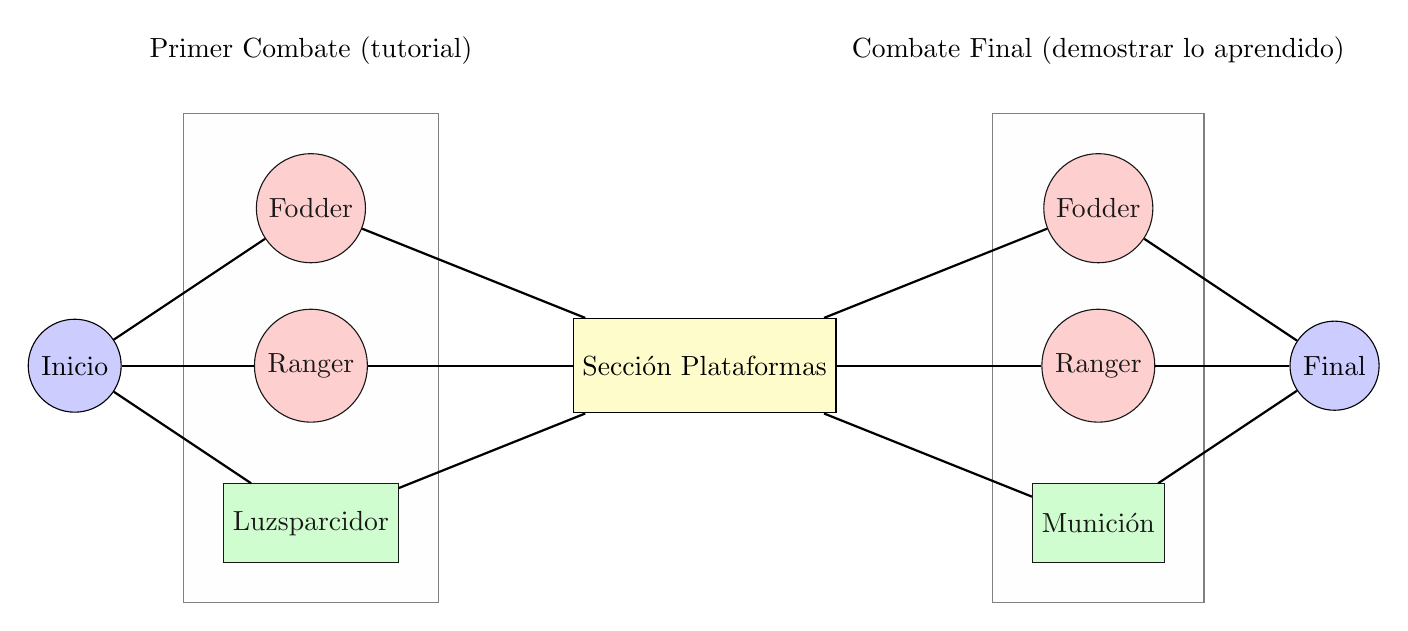
\begin{tikzpicture}
                \usetikzlibrary{fit}
                % Define styles for different elements
                \tikzstyle{player} = [circle, draw, fill=blue!20, minimum size=10mm]
                \tikzstyle{enemy} = [circle, draw, fill=red!20, minimum size=10mm]
                \tikzstyle{item} = [rectangle, draw, fill=green!20, minimum size=10mm]
                \tikzstyle{section} = [rectangle, draw, fill=yellow!20, minimum size=12mm]
                \tikzstyle{path} = [draw, thick, -]
                \tikzstyle{background} = [rectangle, draw=gray, fill=gray!10, inner sep=0.5cm, fill opacity=0.1]

                % Draw the modified layout
                \node[player] (start) at (0,0) {Inicio};

                % First group
                \node[enemy] (enemy1) at (3,2) {Fodder};
                \node[enemy] (enemy2) at (3,0) {Ranger};
                \node[item] (item1) at (3,-2) {Luzsparcidor};

                % Platform section
                \node[section] (platform) at (8,0) {Sección Plataformas};

                % Final combat group
                \node[enemy] (enemy3) at (13,2) {Fodder};
                \node[enemy] (enemy4) at (13,0) {Ranger};
                \node[item] (item2) at (13,-2) {Munición};

                \node[player] (end) at (16,0) {Final};

                % Draw background sections after shapes are defined
                \node[background, fit=(enemy1) (enemy2) (item1)] {};
                \node[background, fit=(enemy3) (enemy4) (item2)] {};

                % Connect the nodes
                \draw[path] (start) -- (enemy1);
                \draw[path] (start) -- (enemy2);
                \draw[path] (start) -- (item1);
                \draw[path] (enemy1) -- (platform);
                \draw[path] (enemy2) -- (platform);
                \draw[path] (item1) -- (platform);
                \draw[path] (platform) -- (enemy3);
                \draw[path] (platform) -- (enemy4);
                \draw[path] (platform) -- (item2);
                \draw[path] (enemy3) -- (end);
                \draw[path] (enemy4) -- (end);
                \draw[path] (item2) -- (end);

                % Add labels with higher y-coordinates
                \node at (3, 4) {Primer Combate (tutorial)};
                \node at (13, 4) {Combate Final (demostrar lo aprendido)};
            \end{tikzpicture}
            }

\newpage

\section{Diseño de Sonido}
    Antes de comenzar esta sección, todos los sonidos enlazados en esta sección se encuentran en esta carpeta de Google Drive, para acceder más todos los archivos fácilmente, no obstante, todos los sonidos estan enlazados individualmente.
        \begin{center}
            \href{https://drive.google.com/open?id=13Drehn-OJeRZ-eS3PpO_D1z_Fl79qpGu&usp=drive_fs}{Enlace a propuesta de sonidos para \gameTitle}
        \end{center}
    \subsection{Banda Sonora} \label{ost}
        La música sería una mezcla de música ambiental pesada y monótona similar a los juegos de terror en las secciones entre batallas. El combate utilizará una mezcla de estos sonidos monótonos pero con \textit{música}. La principal inspiración del estilo de la música es el juego \textbf{\textbf{CULTIC}} \cite{cultic2022} \cite{jasozz_cultic_2023}. La música que podría acompañar al primer nivel, por ejemplo \footnote{ver referencias en \ref{levelDesign}} serían:
            \begin{itemize}
                \item \href{https://youtu.be/LXxBT9cmWjI?si=1Fgiadgp8nBzD8x4&t=245}{3. The Grave (E1M1)}: Esta canción está acompañada de un piano con una melodía melancólica, mientras que en el fondo se puede escuchar guitarreo de fondo; después viene un ritmo que casi parece una marcha fúnebre; o incluso una procesión militar. Esta canción sería ideal para la introducción del juego.
                \item \href{https://youtu.be/LXxBT9cmWjI?si=d9kko76w1qNqges7&t=469}{4. Unstopable (E1M2)}: Esta canción contiene un ritmo similar pero cambia el tono melódico por percusión agresiva y pesada, junto al guitarreo que vez en cuando acompañaba a la canción anterior. Esta canción sería ideal para los combates del primer nivel.
            \end{itemize}
        Se añadiría un tono al finalizar un nivel: \href{https://www.youtube.com/watch?v=LXxBT9cmWjI&t=4407s}{Level End Theme}

        Además, se gestionaría dinámicamente, según el estado donde se encuentra el jugador y que está haciendo; si está explorando es preferible usar una música más calmada, manteniendo cierta tensión para que el jugador siga alerta (para encajar la narrativa con el sonido); y en combate se usaría la misma canción con \textit{layers}, es decir, se añadirían más instrumentos a la canción para el combate.

        Las canciones del modo superviviencia de \textit{\textbf{CULTIC}}, irían perfectamente en el modo \textit{Versus}\ref{versus} de \TWD, ya que la tensión y la velocidad de la música se ajusta perfectamente a la velocidad de juego y la tensión que se quiere transmitir en este modo.
        \begin{itemize}
            \item \href{https://www.youtube.com/watch?v=LXxBT9cmWjI&t=3835s}{\textit{Survival Combat 1 - CULTIC Official Soundtrack}}
            \item \href{https://www.youtube.com/watch?v=LXxBT9cmWjI&t=3931s}{\textit{Survival Combat 2 - CULTIC Official Soundtrack}}
            \item \href{https://www.youtube.com/watch?v=LXxBT9cmWjI&t=4075s}{\textit{Survival Combat 3 - CULTIC Official Soundtrack}}
            \item \href{https://www.youtube.com/watch?v=LXxBT9cmWjI&t=4219s}{\textit{Survival Combat 4 - CULTIC Official Soundtrack}}
            \item \href{https://www.youtube.com/watch?v=LXxBT9cmWjI&t=4315s}{Para la pantalla de resultados / \textit{Survival Results - CULTIC Official Soundtrack}}
        \end{itemize}
    \subsection{Sonido Ambiental}
    Como se menciona en \ref{ost}, el sonido ambiental desempeña un papel clave en la inmersión del jugador dentro del juego. Este tipo de sonido busca transmitir la atmósfera opresiva y tensa del entorno, utilizando elementos como ecos distantes, crujidos, viento, goteos, y otros sonidos sutiles que generan un constante estado de alerta.

    Algunos ejemplos para el \textit{ambience} del nivel:
    \begin{itemize}
        \item \href{https://drive.google.com/open?id=1-BAV8BI2FhwryOpE2sznbGjXXjKJc67C&usp=drive_fs}{Opcion 1 - Quizás escesiva, pero con bastante tensión}
        \item \href{https://drive.google.com/open?id=1-IY4kPhNsTwj1qDsUoW82h4YJGS7cgLj&usp=drive_fs}{Opcion 2 - Más elementos de terror, con un sonido como si fuese respiración}
        \item \href{https://drive.google.com/open?id=1-MlHY4gsA-Nj3UdmaBdFvPJ8E1NEC-u2&usp=drive_fs}{Opcion 3 - Sonido de caverna, con eco y goteo y sonidos como hubiesen una ''presencia''}
    \end{itemize}

    \subsection{Sonido de Mecánicas}
        Los sonidos desempeñan un papel muy importante en el juego. La visión y la luz son los recursos más utilizados, pero cada criatura haría un sonido distinto dependiendo de lo que esté haciendo. Por ejemplo, un enemigo básico haría un gruñido al acercarse al jugador y cuando realiza un ataque de salto, el monstruo anticiparía este ataque haciendo un sonido distintivo. Esto empodera al jugador al no hacerlo depender solo de la luz y el apuntado.
        Algunos ejemplos para los sonidos para las armas:
        \begin{itemize}
            \item \textbf{Luminador:} Un sonido de disparo rápido y agudo, similar a un láser.
            \begin{itemize}
                \item \href{https://drive.google.com/open?id=1--GmmPExYlCoyFkUiGgEEhoB6ZvPko4W&usp=drive_fs}{Opcion 1} - Sonido más tradicional
                \item \href{https://drive.google.com/open?id=1-8QOVx0icIXQ2tiE5wcexUUpAmHtnrhO&usp=drive_fs}{Opcion 2} - Más similar a un láser
            \end{itemize}
            \item \textbf{Luzsparcidor:} Un sonido de disparo más pesado y metálico, con un eco de los perdigones al disparar.
            \begin{itemize}
                \item \href{https://drive.google.com/open?id=1ePwIRZERfeH8iIn4U1qDEDvSef1qM3Ja&usp=drive_fs}{Opcion 1} - Sonido con más impacto
                \item \href{https://drive.google.com/open?id=1d05kAcgOKx4CygJESJ_SjWyzid2VOUDn&usp=drive_fs}{Opcion 2} - Sonido más suave y con más eco
            \end{itemize}
            \item \textbf{Fotón:} Un sonido de carga y descarga de energía, seguido de un disparo profundo y resonante.\\
                \href{https://drive.google.com/open?id=1-6RLC8SU9PWc3WL4-Esuh9aY8DqgYpkp&usp=drive_fs}{Sonido escogido} - Contiene ambos elementos
        \end{itemize}

        % https://drive.google.com/open?id=1-Q6D-lYbQ08UV0V2YRYh_UzvoASzTDrT&usp=drive_fs
        %https://drive.google.com/open?id=1-RnyeL0Zham_IY5yZCOLxoxnW-wHrhX1&usp=drive_fs
        %https://drive.google.com/open?id=1-SIBq_0QMMFYzFxj3VXAsfGzK31PZcJF&usp=drive_fs

        Y algunos sonidos de ejemplo para las criaturas \fodder:
        \begin{itemize}
            \item \href{https://drive.google.com/open?id=1-Q6D-lYbQ08UV0V2YRYh_UzvoASzTDrT&usp=drive_fs}{Opcion 1} - Dañado
            \item \href{https://drive.google.com/open?id=1-RnyeL0Zham_IY5yZCOLxoxnW-wHrhX1&usp=drive_fs}{Opcion 2} - Acechando
            \item \href{https://drive.google.com/open?id=1-SIBq_0QMMFYzFxj3VXAsfGzK31PZcJF&usp=drive_fs}{Opcion 3} - Ataque
        \end{itemize}
\newpage

\section{Diseño de Gamificación}
    % TODO: Hay que crear un sistema
    % https://chatgpt.com/g/g-zhYp7vLsA-gamifica-lo-que-quieras
    \subsection{Objetivos}
    \begin{itemize}
        \item \textbf{Progresión del \hunter:} Implementar un sistema de experiencia que permita al jugador mejorar sus habilidades y estadísticas a medida que avanza en el juego.
        \item \textbf{Dominio de armas:} Crear un sistema de maestría para cada arma (Luminador, Luzsparcidor, Fotón) que recompense el uso constante y efectivo. Esta maestría se mediría según el número de enemigos eliminados, precisión de disparo y uso de habilidades secundarias.
        \item \textbf{Exploración del \hole:} Incentivar la exploración completa de los niveles, recompensando a los jugadores por descubrir secretos y áreas ocultas.
    \end{itemize}

    \subsection{Conflictos}
    \begin{itemize}
        \item \textbf{Gestión de recursos:} Crear tensión entre el uso de munición para atacar y para iluminar, forzando al jugador a tomar decisiones estratégicas.
        \item \textbf{Visibilidad vs. vulnerabilidad:} Establecer un conflicto entre la necesidad de iluminar para ver a los enemigos y el riesgo de ser más visible y vulnerable.
        \item \textbf{Velocidad vs. precisión:} Desafiar al jugador a equilibrar la rapidez de movimiento con la precisión de los disparos, especialmente en situaciones de baja visibilidad.
    \end{itemize}

    \subsection{Mecánicas}
    \begin{itemize}
        \item \textbf{Sistema de combos de luz:} Recompensar al jugador con puntos extra o bonificaciones por encadenar eliminaciones de enemigos usando hábilmente las mecánicas de luz.
        \item \textbf{Desafíos diarios:} Implementar misiones diarias que reten al jugador a completar objetivos específicos, como eliminar cierto número de enemigos con un arma particular o completar un nivel sin usar bengalas.
        \item \textbf{Coleccionables de lore:} Dispersar notas y artefactos por los niveles que revelen más sobre la historia del mundo, incentivando la exploración y recompensando a los jugadores con conocimiento adicional.
        \item \textbf{Sistema de rangos de \hunter:} Crear un sistema de rangos que el jugador pueda subir al completar misiones y demostrar habilidad, desbloqueando nuevas personalizaciones o habilidades.
        \item \textbf{Modo Endless mejorado:} Expandir el modo Endless con un sistema de leaderboards y recompensas únicas basadas en la puntuación y el tiempo de supervivencia.
    \end{itemize}

\newpage

\section{Diseño de Monetización}
% Hay que ponerle un apartado de diseño de monetizacion. Hay que proponer todos los sistemas que sean lógicos para el juego.
    Debido a que \gameTitle es un juego primariamente de un jugador con un modo multijugador a modo de acompañamiento \textit{(ver sección \ref{multiplayer})}, la monetización se centrará en la venta del juego base y expansiones de contenido adicional.

    A continuación, se detallan los métodos de monetización que se consideran aplicables\footnote{basado en el documento: \textit{Gamification Design del AV}} a \gameTitle y se describen cómo se implementarían en el juego.

    \begin{table}[H]
        \resizebox{\textwidth}{!}{%
        \begin{tabular}{@{}|l|l|l|@{}}
            \toprule
            \textbf{\textit{Método de Monetización}}       & \textbf{\textit{¿Aplicable a \TWD?}} & \textbf{\textit{Descripción}}                                               \\ \midrule
            \textbf{Pay to play}                           & Sí                     & Venta del juego base a precio fijo                                 \\ \midrule
            \textbf{DLC}                                   & Sí                     & Expansiones con nuevos niveles, armas o enemigos                   \\ \midrule
            \textbf{Virtual goods (cosmetics)}             & Sí                     & Skins para armas, efectos visuales personalizados                  \\ \midrule
            \textbf{Season Pass}                           & Sí                     & Acceso a futuros DLCs y contenido exclusivo                        \\ \midrule
            \textbf{Founder pack}                          & Sí                     & Edición especial para primeros compradores                         \\ \midrule
            \textbf{Virtual goods (advance, power ups)}    & Limitado               & Mejoras temporales para modo Endless                               \\ \midrule
            \textbf{Merchandising}                         & Sí                     & Productos físicos relacionados con el juego                        \\ \midrule
            \textbf{Free to play version}                  & Limitado               & Versión limitada del modo Endless                                  \\ \midrule
            \textbf{Trial}                                 & Sí                     & Primer capítulo de la campaña gratuito (a modo de demo)            \\ \midrule
            \textbf{Pay for multiplayer}                   & Potencial              & Si se implementa modo multijugador                                 \\ \midrule
            \textbf{In-game advertising}                   & No                     & No se ajusta al estilo del juego                                   \\ \midrule
            \textbf{Pay to avoid ads}                      & No                     & No hay anuncios que evitar                                         \\ \midrule
            \textbf{Pay to avoid waiting}                  & No                     & No se ajusta al diseño del juego                                   \\ \midrule
            \textbf{Virtual goods (advantage competition)} & No                     & Podría desbalancear el juego                                       \\ \midrule
            \textbf{Freemium Games}                        & No                     & No se ajusta al modelo del juego                                   \\ \midrule
            \textbf{Crowdfunding}                          & Potencial              & Para futuras expansiones o secuelas                                \\ \midrule
            \textbf{Pay subscription}                      & No                     & No se ajusta al modelo del juego                                   \\ \midrule
            \textbf{Display advertising}                   & No                     & No se ajusta al estilo del juego                                   \\ \midrule
            \textbf{NFT}                                   & No                     & No se ajusta al concepto del juego                                 \\ \midrule
            \textbf{Arcade machines}                       & No                     & No aplicable para este tipo de juego                               \\ \bottomrule
        \end{tabular}%
        }
        \caption{Monetización de \gameTitle}
        \label{tab:monetization}
    \end{table}

\newpage

\section{Diseño del Multijugador} \label{multiplayer}
    % DONE: Crear una narrativa para el multijugador. A emilio le interesa.
    % En el mundo se hacen quizás combates amistosos para entrenar a los cazadores, o incluso se hacen competiciones para ver quién es el mejor cazador.
    En \gameTitle, se introducen dos modos distintos de juego para el multijugador, siendo estos complementarios a la campaña. Es decir, el modo campaña sería el modo principal de juego mientras que el multijugador es un ''añadido''; por ejemplo, en \textit{Gears Of War} \cite{gearsofwar2006}, donde el juego se ofrecía el modo campaña como el modo principal, y el multijugador como un modo complementario.

    Esto era una práctica muy común en juegos anteriores a la séptima generación de consolas \footnote{Xbox 360, PS3, Wii}; como ejemplo añadido, en \textit{Unreal Tournament} \cite{unrealtournament1999} se empezó a ofrecer un modo campaña en entregas posteriores, siendo este un juego exclusivamente multijugador. \cite{quake1996} también ofrecía un modo campaña, pero este era más un añadido que el modo multijugador.

    Pasando de nuevo a \gameTitle, se seguirá esta misma filosofía.
    \subsection{Implementación de la Historia}
        Para integrar la historia con el multijugador, los \hunters tendrían arenas de práctica donde se enfrentarían entre ellos para mejorar sus habilidades y competir por el rango de mejor \hunter. Estas arenas estarían situadas en lugares clave de \hole, donde los \hunters se reunirían para entrenar y competir.
        \begin{itemize}
            \item \textbf{Torneos de \hunters:} Organizar torneos periódicos donde los \hunters compiten por recursos escasos o por el derecho a liderar misiones importantes.
            \item \textbf{Misiones de Entrenamiento:} Crear escenarios de entrenamiento que simulen condiciones reales de \hole, permitiendo a los \hunters practicar en un entorno controlado.
            \item \textbf{Rangos y Reputación:} Implementar un sistema de rangos que refleje la habilidad y experiencia de los \hunters, influenciando su posición en la sociedad y el acceso a misiones más prestigiosas.
        \end{itemize}
    \subsection{Modo Coperativo}
        En el modo cooperativo, se permitiría a los jugadores completar misiones de la campaña juntos, con la dificultad ajustada para dos jugadores. Además, el modo cooperativo incluría la posibilidad de asignar roles o clases a los jugadores que se especialicen en roles específicos como ''iluminador'' o ''francotirador'', fomentando la cooperación estratégica.
    \subsection{Modo \textit{Versus}} \label{versus}
        Se seguiría la estructura básica de \textit{Quake} y \textit{Halo} \cite{halo2001}, donde los jugadores se enfrentan en una arena de tamaño variable, donde nadie empezaría con armas equipadas y los jugadores tendrían que encontrarlas en el mapa, en sitios estratégicos.
        \begin{itemize}
            \item Modos de Juego Únicos:
            \begin{itemize}
                \item \textbf{''Caza en la Oscuridad'':} Los jugadores comienzan en total oscuridad y deben usar la luz estratégicamente para localizar y eliminar oponentes.
                \item \textbf{''Captura la Llama'':} Una variación de captura la bandera donde el objeto a capturar es una fuente de luz.
            \end{itemize}

            \item Mecánicas de Luz en Versus:
            \begin{itemize}
                \item Zonas de oscuridad que ocultan a los jugadores.
                \item Armas que temporalmente cegan a los oponentes.
                \item Powerups que aumentan la visibilidad del jugador o reducen la de los oponentes.
            \end{itemize}
            \item \textbf{Mapas Dinámicos:} Crear mapas con elementos interactivos que afecten la iluminación, como generadores que pueden ser activados o desactivados.
            \item \textbf{Modos Asimétricos: }Un equipo juega como \hunters y otro como criaturas de la oscuridad, cada uno con habilidades únicas.
        \end{itemize}
